\setchapterpreamble[u]{\margintoc}

\chapter{Droplet Generation in Corrugated Ligaments}
\labch{breakup}

% Rearrangement of liquid volumes in ligaments
Ligaments constitute the penultimate stage in the complex sequence 
of capillary-driven topological changes that are 
typical of liquid fragmentation processes, 
finally resulting in the generation of polydisperse collections of drops. 
In the context of the present body of work, we shall 
only concern ourselves with the dynamics of Newtonian ligaments, 
which are well described by the Navier-Stokes equations 
at the incompressible and isothermal limits. 
The rearrangement of the liquid volumes that constitute
the ligaments play a key role in determining the size 
of the droplets that emerge immediately after the disintegration
of the thread-like structure (Fig. \ref{lig_stretch} ).  

\begin{marginfigure}[3cm]
\centering
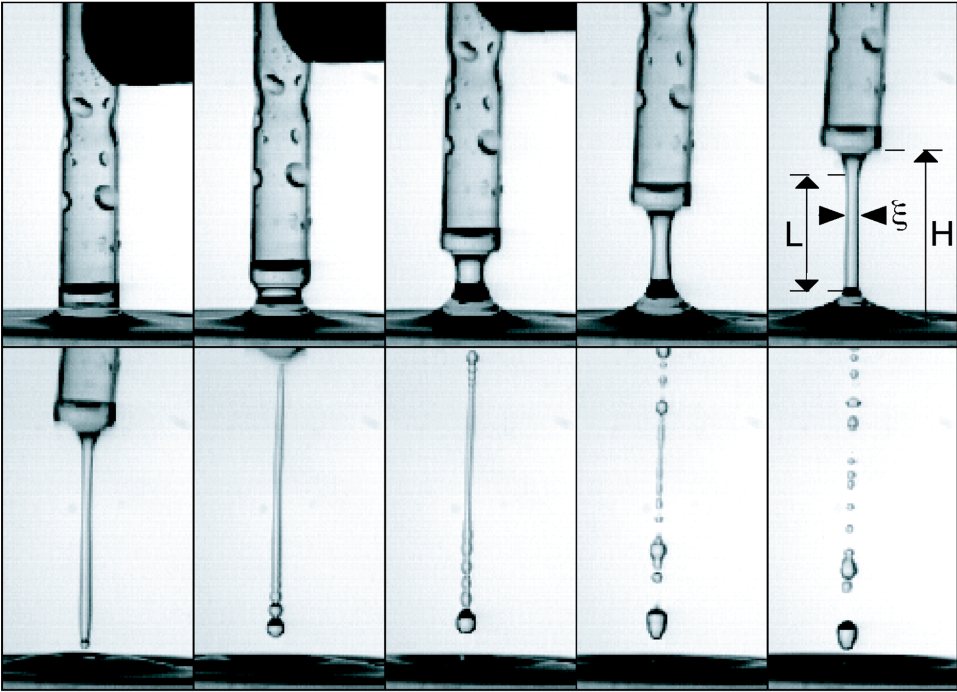
\includegraphics{plots/ligament_breakup/lig_mar_vill_pof04.png}
\caption{Fragmentation of stretched liquid (Newtonian) ligaments, reproduced 
	from Marmottant \& Villermaux \cite{vill_3}.
       	The complex rearrangement of the liquid volumes 
	inside the ligament results in its disintegration 
	into droplet of various sizes. 
	}
\label{lig_stretch}
\end{marginfigure}

The dynamics of these rearrangements prior to breakup are 
governed by non-linear interactions between several 
physical mechanisms such as the growth and propagation of capillary 
waves along the ligament surface, remnants of the internal flow, 
stretching induced either by the surrounding gas flow or by 
acceleration of the liquid into the surrounding medium itself,
not to mention the dissipative effects of viscosity.  
Although we present a convoluted picture of ligament dynamics prior
to breakup, it is ultimately the capillary force that drives the 
eventual topology change from the thread-like structure to that of the drop. 
The primary role of the both the inertial and viscous forces is to oppose 
or dampen the destabilizing effects of the capillarity induced deformations.   
An additional mechanism to consider is the merger or coalescence of the 
newly created droplets (post-breakup) along the axis of the former ligament
structure, or with droplets originating from other sources in the near vicinity. 
The generation of drops whose diameters are significantly larger than the 
width of original ligament are predominantly driven by the aforementioned coalescences.  
Therefore, considering the combined effects of the above mechanisms, we expect a significant
departure of the resulting drop size distribution from that predicted by the  
classical analysis of the Rayleigh-Plateau instability \cite{rayleigh1879a,rayleigh1879b}. 


% Corrugation-coalescence model
Linear theory based on the the Rayleigh breakup of infinitely
long liquid cylinders in a quiescent medium predicts the disintegration
of the thread along regular intervals, the length of which is governed
by the fastest growing spatial frequency. 
The drops generated according to this model would be uniform in
size, in sharp contrast to the significant variances in the size distributions
observed in reality.  
Even in the simpler case of decaying liquid jets, 
non-linearities near the breakup zone kick into effect beyond
the initial exponential growth phase predicted by linear theory, 
eventually resulting in the jet breaking up into 
``main'' drops and significantly smaller ``satellite'' droplets 
\sidenote{Refer to the high quality photographs in 
the work of Rutland and Jameson \cite{rutland1971non}, where they demonstrate 
the formation of ``satellite'' droplets that manifest due to the non-linear effects
driving the jet breakup.}. 
Thus, simply taking into account the non-linear effects driving the breakup would
lead to a bimodal distribution of droplet size, but this explanation 
still fails to account for the broad distribution of sizes observed in 
the outcomes of the majority of natural \cite{nature} and industrial \cite{industrial} processes. 


As we have seen in the previous chapter, there are several hypotheses 
in existing literature \sidecite{vill_1} 
that attempt to model the underlying physical mechanisms 
that are responsible for the selection of droplet size. 
A model first proposed by Villermaux and coworkers \sidecite{vill_2,vill_4}
asserts that the variance in the droplet sizes is strongly 
correlated to the initially corrugated shape of the 
ligament, from which the drops originate. 
In this model, the corrugated ligament is represented as a collection 
of `blobs' (see Fig. \ref{blobs}), with the continuous interaction between 
such blobs throughout the destabilization phase accounting for the 
rearrangement and concomitant aggregation of the liquid volumes prior to breakup. 
\marginnote{
The corrugation-coalescence mechanisn has been 
popularized in several studies such as \cite{vill_3,vill_1,vill_5,vill_6,vill_7},
and more recently in \cite{bonn,mckinley}.
}
The key parameter concerning the predictions of this model 
is $n$, which characterizes the corrugations in the initial 
geometrical shape of the ligament, defined as  

\begin{align}
	n \equiv \frac{1}{\left(\langle d^{2} \rangle - \langle d \rangle^{2} \right) / \langle d \rangle^{2}}
\end{align}

where the quantities in the brackets $\langle \quad \rangle$ represent the mean
and the diameters $d_i$ correspond to that of the blobs as shown in Fig. \ref{blobs}.
These studies essentially demonstrate that the degree of polydispersity 
in the drop sizes can be simply explained by examining the 
degree of ``smoothness'' in the initial geometry of the ligaments, 
with the standard deviation or distribution width of the size of the 
emerging drops scaling as $1 / \sqrt{n}$. 
As a corollary to this prediction, a broader distribution of drop sizes arise out
of the disintegration of strongly corrugated (rough) ligaments, whereas smoother 
ligaments with uniform thickness lead to a narrower (monodisperse) distributions. 

\begin{marginfigure}
\centering
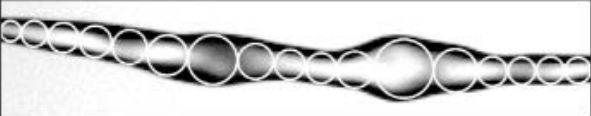
\includegraphics{plots/ligament_breakup/lig_protoblobs.png}
\caption{Representation of the liquid volumes in an isolated ligament as `blobs'
	of sizes $d_0$ corresponding to the local thickness,
	,reproduced from Villermaux \cite{vill_1}.
	}
\label{blobs}
\end{marginfigure}




% Difficulties associated 



%Due to the complex nature of such fragmentation processes, 
%it has proven to be quite a difficult challenge for both 
%experimental and numerical studies to establish the 
%mechanistic link between the initial surface corrugations 
%and the resulting drop size distributions.  
%
%
%In the present study, we have developed a numerical experiment 
%that grants us precise control over both quantitative and 
%qualitative aspects of such random corrugations, and its subsequent 
%influence on the resulting droplet sizes. 



\section{Breakup Regimes}

% Brief review, eggers , Keller-Miksis and Viscous regimes


%---------------------------------------------------------------
\section{Numerical Setup}
We perform direct numerical simulations of the two-phase 
Navier-Stokes equations under the incompressible framework. 
Material properties correspond to that of air-water systems at 20 degrees Celsius. 
Simulations are carried out in the axi-symmetric framework, 
therefore excluding the existence of azimuthal modes with 
respect to the central axis of the ligament. 

\paragraph{Platform : Basilisk}
\blindtext

\paragraph{Computational Schematic}
\blindtext

\paragraph{Random Surface Generation}
\blindtext

\paragraph{Parameterization}
\blindtext

\paragraph{Quantization of Waves}
\blindtext

%---------------------------------------------------------------

\section{Impact of Initial Conditions}

\paragraph{3D vs. 2D Simulations}
\blindtext

\paragraph{Effect of Spatial Resolution}
\blindtext

\paragraph{Effect of Droplet Removal}
\blindtext

\paragraph{Effect of Corrugation Amplitude}
\blindtext

\paragraph{Effect of Ohnesorge Number}
\blindtext

\paragraph{Effect of Cut-Off Wavenumber}
\blindtext

\paragraph{Effect of Aspect Ratio}
\blindtext


